\documentclass{beamer}

\usepackage{xcolor}
\usepackage{tikz}

\usetikzlibrary{calc, tikzmark, arrows, shapes, positioning, backgrounds}
\tikzset{every picture/.style={remember picture}}

\usepackage{xcolor}

% MATLAB colors
\definecolor{matlab-blue}{rgb}{0.0000, 0.4470, 0.7410}
\definecolor{matlab-red}{rgb}{0.8500, 0.3250, 0.0980}
\definecolor{matlab-yellow}{rgb}{0.9290, 0.6940, 0.1250}
\definecolor{matlab-purple}{rgb}{0.4940, 0.1840, 0.5560}

% NTNU colors
\definecolor{ntnu-blue}{RGB}{0, 80, 158}

% SINTEF colors
% \definecolor{sintef-green}{RGB}{0,172,160}
\definecolor{sintef-gray}{RGB}{51,51,51}
\definecolor{sintef-blue}{RGB}{0,61,101}

% Phase colors
\definecolor{aqu}{RGB}{95 ,  95, 211}
\definecolor{liq}{RGB}{145, 124, 111}
\definecolor{rock}{RGB}{179, 179, 179}

% Code
\colorlet{codecolor}{matlab-yellow!6}

\usepackage{pgfplots}

\usepackage[active,tightpage]{preview}
\PreviewEnvironment{tikzpicture}
\setlength\PreviewBorder{0pt}

\usepackage{amsmath, amsfonts, amssymb}
\usepackage[outdir=./]{epstopdf}

\usepackage{tikz}
\usetikzlibrary{calc, tikzmark, arrows, shapes, positioning, backgrounds}

% Figure styles
\tikzstyle{fig} = [anchor = west, inner sep=0]
\tikzstyle{label} = [anchor = north, inner sep=0]
\tikzstyle{label2} = [draw, rectangle, rounded corners, fill=white, anchor = north west, align = center, minimum height = 1.8em]

% Drawing styles
\tikzstyle{line} = [line width = 1.5pt]
\tikzstyle{sline} = [line width = 0.2pt]
\tikzstyle{dline} = [line width = 0.1pt, dashed]
\tikzstyle{zline} = [line width = 0.5pt, dashed]
\tikzstyle{tline} = [line width = 2pt]

% Box styles
\tikzstyle{explain} = [rectangle, draw = black, fill=black!10, rounded corners, font = \small, thick, text centered, minimum height = 1.7em]
\tikzstyle{block} = [rectangle, draw = black, fill=black!10, rounded corners, font = \small\bfseries, thick, text centered, minimum height = 1.7em, anchor = north, line width = 0.5pt]
\tikzstyle{eblock} = [rectangle, draw = black, rounded corners, font = \small, thick, text centered, minimum height = 1.7em, anchor = center, align = left, inner sep = 1em]
\tikzstyle{rblock} = [rectangle, draw = black, fill=matlab-red!80, rounded corners, font = \small, thick, text centered, minimum height = 1.7em, anchor = north]
\tikzstyle{wblock} = [rectangle, draw = white, fill=white, font = \small\bfseries, thick, text centered, minimum height = 1.7em, anchor = west]
\tikzstyle{topic-gray} = [rectangle, draw=black!10, fill=black!10, font = \small, thick, text centered, minimum height = 1.7em, anchor = west, align = left]
\tikzstyle{topic-red} = [rectangle, draw=matlab-red!80, fill=matlab-red!80, font = \small, thick, text centered, minimum height = 1.7em, anchor = west, align = left]
\tikzstyle{presentation-block} = [rectangle, draw=black, fill=sintef-blue!30, font = \small, thick, text centered, minimum height = 1.7em, anchor = west, align = left, rounded corners, align = center]
% \tikzstyle{eblock2} = [rectangle, draw = black, fill=matlab-red!80, rounded corners, font = \small, thick, text centered, minimum height = 1.7em, anchor = north]


\tikzstyle{decision} = [diamond, aspect = 2, draw=black, fill=matlab-blue!20, text centered, minimum height = 1.7em, align = left]


%\tikzstyle{process} = [rectangle, draw=black, fill=matlab-blue!70, font = \normalfont, line width = 1, text centered, minimum height = 1.7em, anchor = west]

% \tikzstyle{eblock2} = [rectangle, draw = black, fill=matlab-red!80, rounded corners, font = \small, thick, text centered, minimum height = 1.7em, anchor = north]


\usepackage{tcolorbox}
\tcbuselibrary{most}
% Main box style
\newtcolorbox{mainblock}[3]{colback=white, colframe=black, fonttitle=\bfseries\centering, title=#1, height=#3, top = 0.5em, bottom = 0.5em, before skip = \boxskip, after skip = \boxskip, fontupper=\color{black}, width = #2, left = 0.1em}%

\newtcolorbox{solver}[3]{colback=bl!20, colframe=black, top = 0.5em, bottom = 0.0em, before skip = 0em, after skip= 0em, colback = matlab-blue!20, colbacklower = matlab-blue!20, width = #1, height = #2, title = #3, fonttitle=\bfseries\centering, rightrule = 0.5pt, leftrule = 0.5pt, toprule = 0.5pt, bottomrule = 0.5pt, titlerule = 0.5pt, colbacktitle=matlab-blue!80}%

\usepackage{amsmath, amsfonts, amssymb, amsthm}



% \newlength{\figwidth}
% \setlength{\figwidth}{160mm}
\setlength{\fboxsep}{0pt}

\usepackage{bm}
\newcommand{\vect}[1]{\bm{#1}}
\newcommand{\vel}{\vec v}
\newcommand{\perm}{K}
\newcommand{\vx}{\vect x}
\newcommand{\spa}{D}
\newcommand{\bhp}{p_{\mathsf{bh}}}
\newcommand{\dd}{\mathsf{d}}

\begin{document}

\begin{tikzpicture}
    
    \newlength{\figwidth}
    \setlength{\figwidth}{0.3\textwidth}
    \newlength{\figsep}
    \setlength{\figsep}{0.1\figwidth}

    % Figures
    \node[fig, inner sep = 0em, opacity = 0.4] (p1) {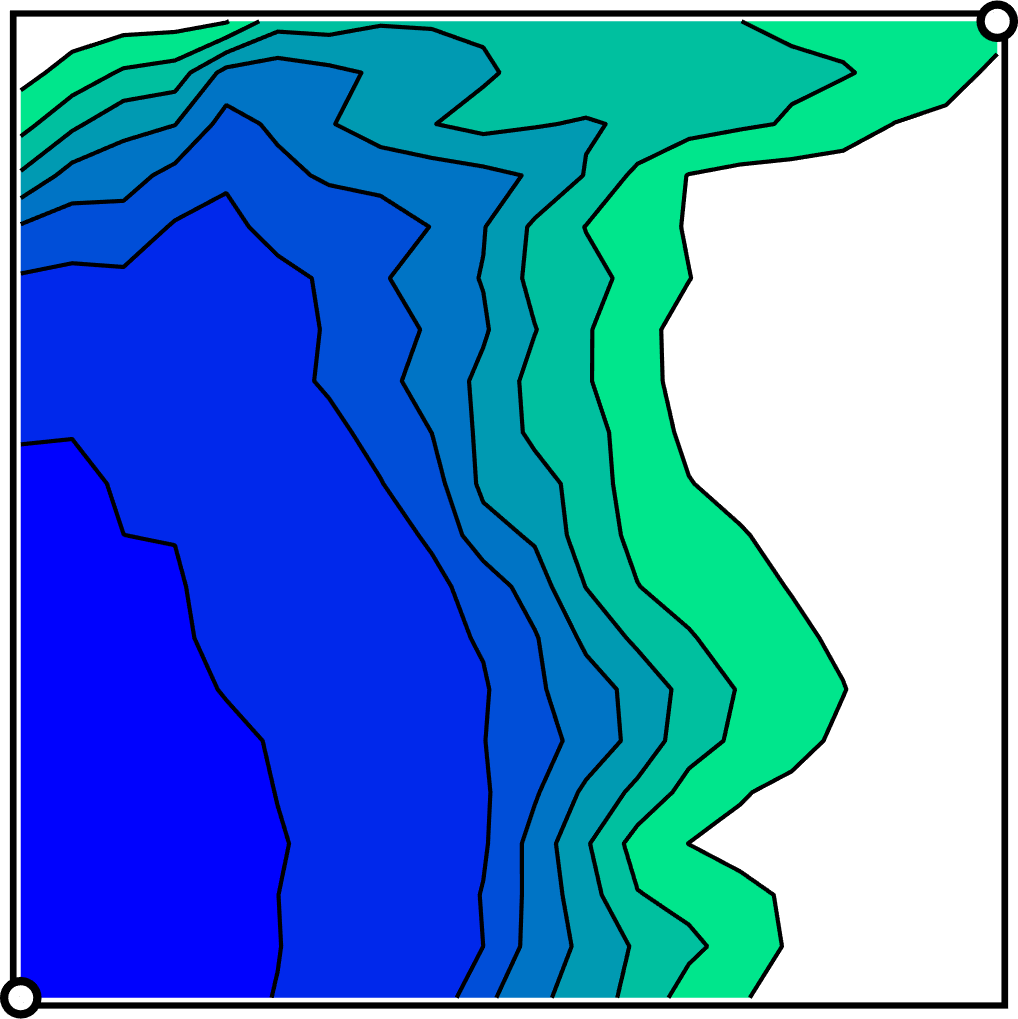
\includegraphics[width = \figwidth]{figures/example-2/sat/sat-1.png}};
    \node[fig, inner sep = 0em, anchor = west, opacity = 0.4] (p2) at ($({p1.east}) + (\figsep, 0)$) {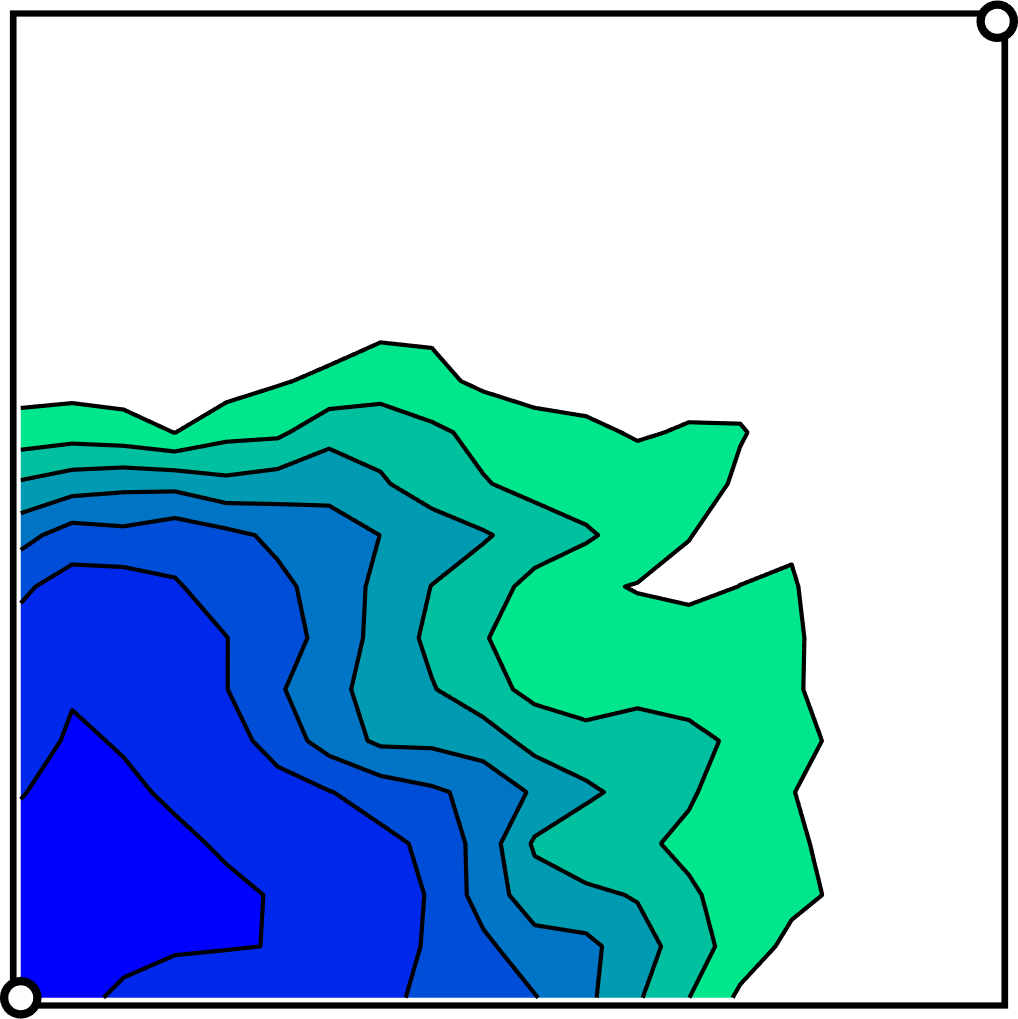
\includegraphics[width = \figwidth]{figures/example-2/sat/sat-2.png}};
    \node[fig, inner sep = 0em, anchor = west, opacity = 0.4] (p3) at ($({p2.east}) + (\figsep, 0)$) {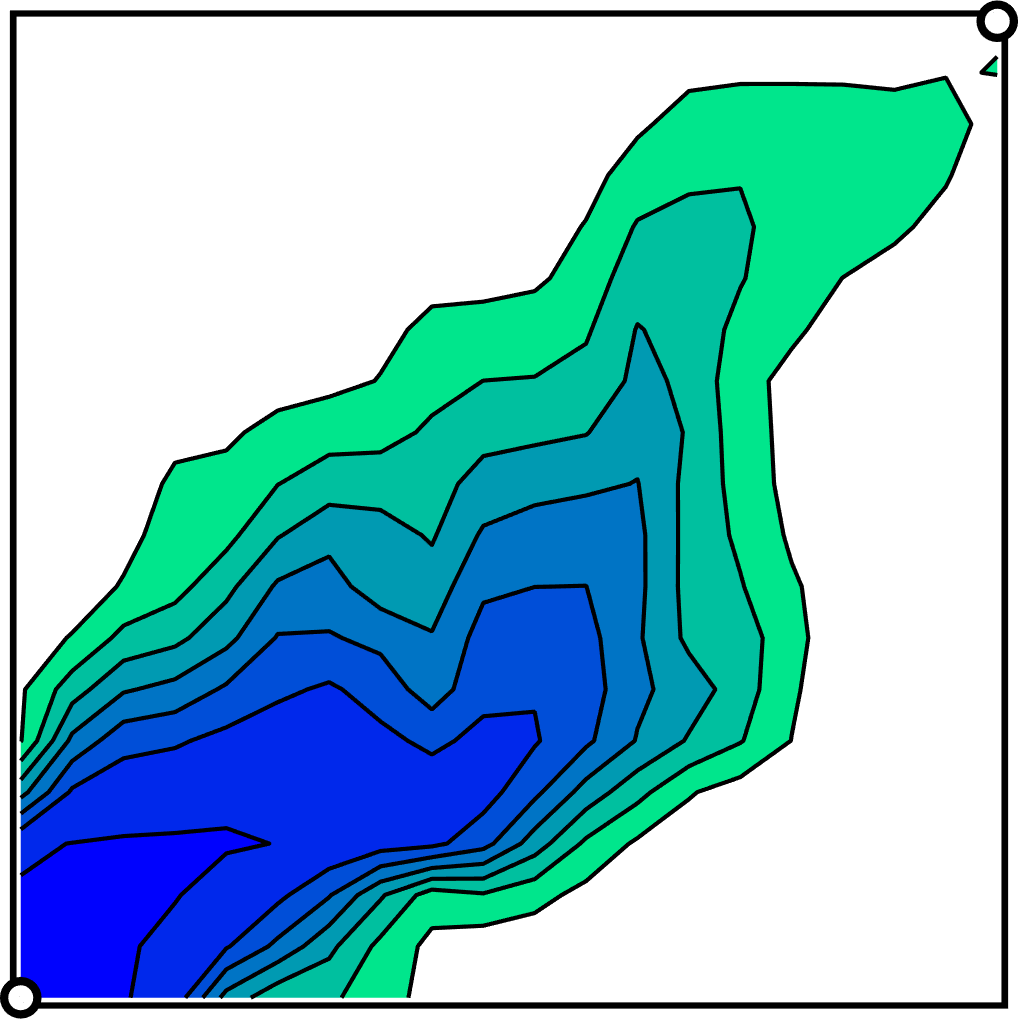
\includegraphics[width = \figwidth]{figures/example-2/sat/sat-3.png}};
    \node[fig, inner sep = 0em, anchor = west] (p4) at ($({p3.east}) + (\figsep, 0)$) {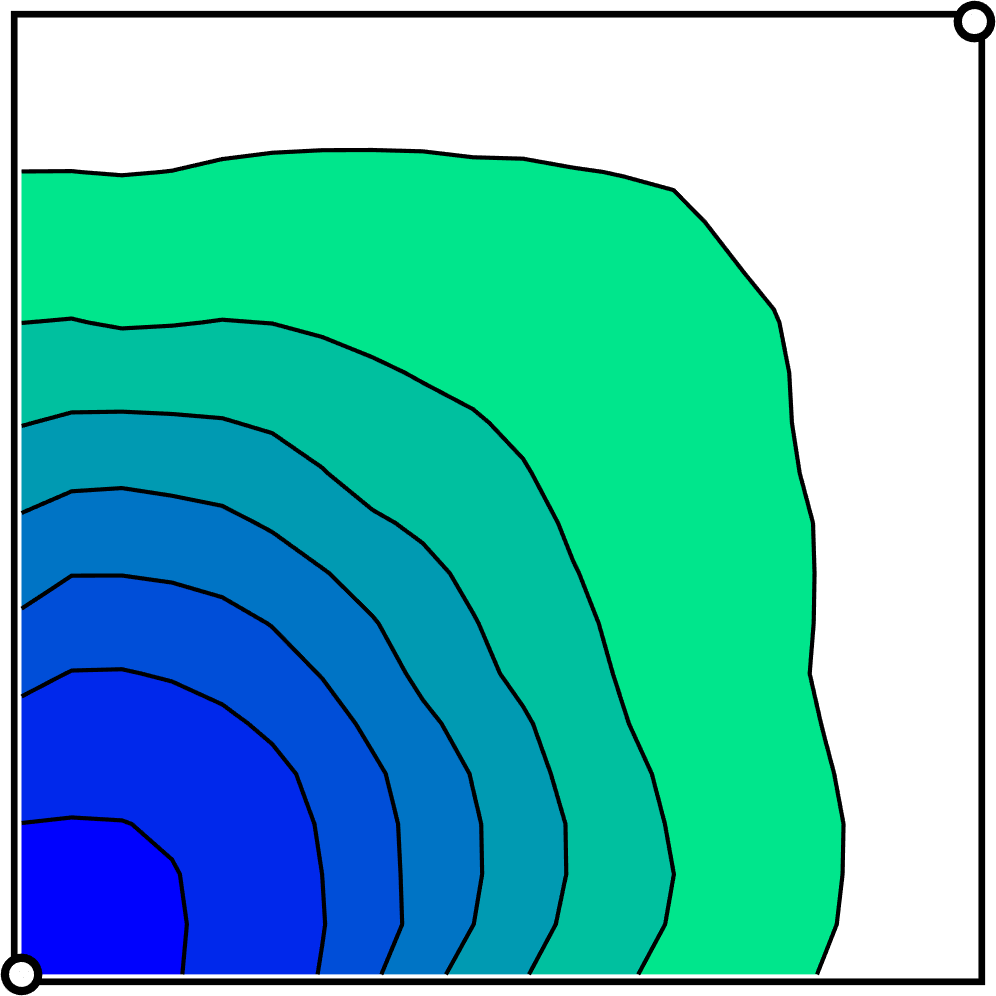
\includegraphics[width = \figwidth]{figures/example-2/sat/sat-mean.png}};
    \node[fig, inner sep = 0em, anchor = south, opacity = 0.4] (p5) at ($({p3.north}) + (0, \figsep)$) {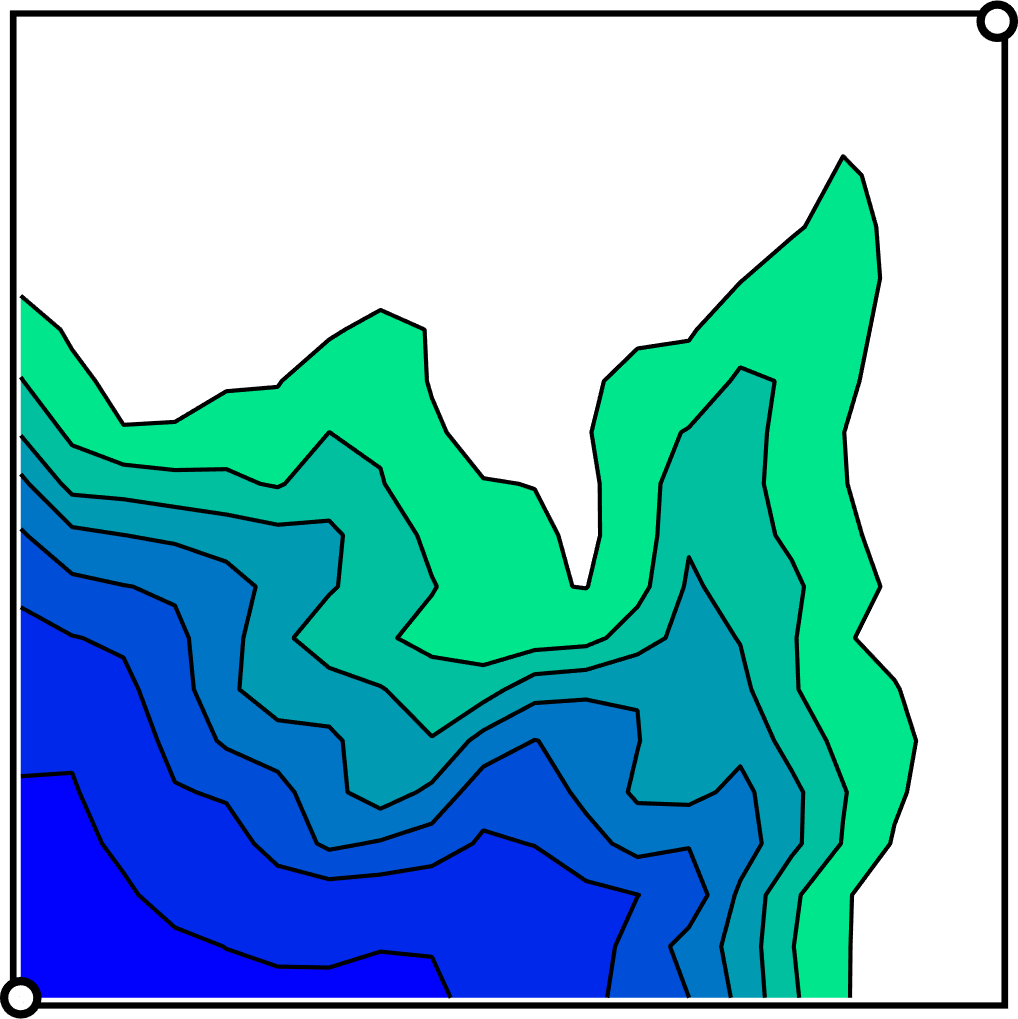
\includegraphics[width = \figwidth]{figures/example-2/sat/sat-5.png}};
    \node[fig, inner sep = 0em, anchor = west, opacity = 0.4] (p6) at ($({p5.east}) + (\figsep, 0)$) {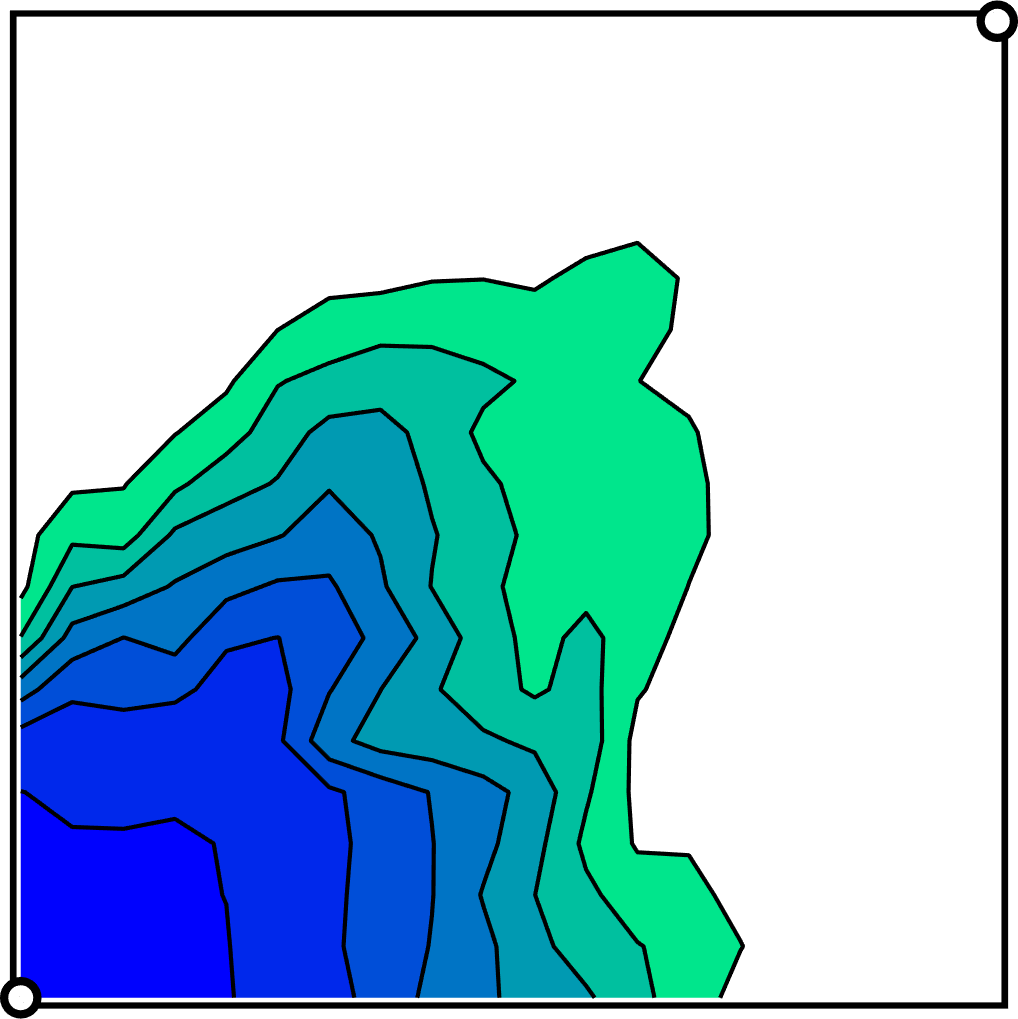
\includegraphics[width = \figwidth]{figures/example-2/sat/sat-6.png}};
    
    \node[label2, anchor = center, minimum width = 2\figwidth] at ($({p1.north}) + (0.5\figsep + 0.5\figwidth, \figsep+0.5\figwidth)$) {%
        \textbf{Covariance function}\\\\
        $\begin{aligned}
            C(\vx, \vx') = \sigma^2 \exp\left(-\frac{\|\vx - \vx'\|}{\lambda}\right)
        \end{aligned}$\\\\
        covariance $\sigma^2 = 1$ \\
        correlation length $\lambda = 0.3$
    };
    
\end{tikzpicture}

\end{document}